\chapter{\SysName アルゴリズム}
本章において,\$1を拡張した\$Vアルゴリズムについて述べる.

\section{\$Vアルゴリズムが目指す特徴}
\$Vアルゴリズムが目指す特徴を以下に示す.
\begin{itemize}
\item \$1の特徴を維持すること.つまり,
\begin{itemize}
\item ハードウェアやソフトウェアのセンシング及び入力する速度などによって変わるサンプリングされる点の数の違いに対してロバストであること.
%\item 手書きジェスチャの大きさ,向き,位置の不変に関してオプショナルに設定可能であること.
\item 数学的な高度な知識やテクニックをを必要としないこと~(例えば,逆行列,微分,積分など)
\item 少ないコードによって実装できること.
\item 認識速度が速いこと.
\item ソフトウェア開発者やアプリケーションユーザが,独自に手書きジェスチャを定義できること.
\item N-best listに関して,高い識別能力を示すスコアを示すこと.
\item 図\ref{fig:stroke_1}のような単一ストロークからなる手書きジェスチャを認識するにあたり,HCI分野において多く用いられる既存の複雑な手書きジェスチャ認識アルゴリズムと比べても,高い認識率を示すこと.
\end{itemize}
\item その上で,形状や書き順が同じ手書きジェスチャを大きさ,向き,位置に関して識別可能にすること.
\end{itemize}

これまで述べてきたように,一般的に,特徴量を不変にすることによってその特徴量についてロバスト性が向上するが,不変せず,認識に用いる特徴量として扱う場合,ロバスト性が低下し,結果的に認識率の低下を招く恐れがある.つまり,\$1アルゴリズムを踏襲した上で,大きさ,向き,位置を特徴量として用い,それらに関して識別可能にするということは,\$1と比べて,認識率が低下すると言っていいだろう.
以上を踏まえ,\$1に比べて,認識率や認識速度を著しく損なうことなく,図のような手書きジェスチャの形状と書き順は同じでも,大きさ,向き,位置が異なるジェスチャを識別するアルゴリズムを実現することが\$Vが目指すところである.

\section{\$Vアルゴリズムのアイディア}

\subsection{大きさ,向き,位置に関して識別可能にする方法}
ジェスチャを大きさ,向き,位置によって識別可能にするための方法として以下の2つが考えられる.
\begin{enumerate}
\item 単純にリサンプリングした点のみによって判別する~(正規化しない).
\item 正規化した上で,それぞれを特徴量として用いる.
\end{enumerate}
1. の場合,リサンプリングしただけの実質生データのまま比較するため,大きさ,向き,位置によって識別可能となる.しかしながら,手書きジェスチャの場合,アプリケーションユーザの入力は毎度微妙に異なることが予想される.そのため,類似したジェスチャにおいても,類似度が低くなり,ロバスト性が大きく低下する恐れがあるとともに,認識されたか否かを判別するための閾値の設定が困難になることが予想される.
2. の場合,ジェスチャを正規化するためロバスト性は維持され,その上で,大きさ,向き,位置を特徴量として用いるため,1. の場合と比べて,類似度が低くなりづらくなると予想される.
そこで,\$Vは2. の方法を用いることとする.

\subsection{学習データの保持の方法}
\$Vは学習データの保持の方法において特徴がある.

\$Vは学習データが追加されるたびに,ジェスチャの形状と書き順が同じ学習データを同じグループに分類する.ここでは形状と書き順が同じジェスチャを識別可能な\$1アルゴリズムを用いている.この形状と書き順に従って分類されたジェスチャを``ジェスチャグループ''と名付ける.

このようにジェスチャグループを作成する理由は2つある.
\begin{itemize}
\item 認識速度の低下を防ぐため.
\item 認識率の低下を防ぐため.
\end{itemize}

「認識速度の低下を防ぐため」について述べる.

大きさ,向き,位置を特徴量として認識に用いる場合,それぞれについての類似度計算を行うこととなる.これを全てのジェスチャについて類似度計算を行った場合,認識速度が低下する要因となる.
\$Vの目的は,ジェスチャの形状と書き順が同じであるが,大きさ,向き,位置に関して識別可能にすることである.そこで,形状と書き順が同じジェスチャが集まったジェスチャグループを作成し,ジェスチャグループ内に存在する学習データのみに対し,大きさ,向き,位置の類似度計算をする.一般的に,認識に用いる特徴量を増やした場合,増やさない場合と比べて,認識速度は学習データの数に比例して大きくなるが,同一ジェスチャグループ内のみに対し認識に用いる特徴量を増やすことによって,全体的な認識速度の低下を防ぐことが可能となる.

次に「認識率の低下を防ぐため」について述べる.

大きさ,向き,位置の特徴量を認識のために全てのジェスチャに対し用いた場合を考える.

例えば,図\ref{fig:cannot_recognized}Aの場合について考える.
学習データ~(図\ref{fig:cannot_recognized})A'が図\ref{fig:cannot_recognized}Aの右下のジェスチャと一致させようと入力されたとする.しかし,この2つのジェスチャは大きさが異なるため,大きさを認識のための特徴量として用いている限り類似度は低下する.

図\ref{fig:cannot_recognized}Bの場合について考える.
学習データ~(図\ref{fig:cannot_recognized})B'が図\ref{fig:cannot_recognized}Bの右のジェスチャと一致させようと入力されたとする.しかし,この2つのジェスチャは向きが異なるため,向きを認識のための特徴量として用いている限り類似度は低下する.

図\ref{fig:cannot_recognized}Cの場合について考える.
学習データ~(図\ref{fig:cannot_recognized})C'が図\ref{fig:cannot_recognized}Cのジェスチャと一致させようと入力されたとする.しかし,この2つのジェスチャは大きさ,向き,位置が異なるため,大きさ,向き,位置を認識のための特徴量として用いている限り類似度は低下する.

これまでに述べてきたが,大きさ,向き,位置を特徴量として認識のために新たに用いることによって,それぞれについてロバスト性が低下し,結果的に認識率の低下を招く恐れがある.図\ref{fig:cannot_recognized}はその例である.

\begin{figure} [h!]
	\begin{center}
		\includegraphics [width=0.9\hsize ]{img/cannot_recognized.eps}
	\end{center}
	\caption{大きさ,向き,位置を特徴量として認識のために用いた場合に,入力データと学習データが一致しない例}
	\label{fig:cannot_recognized}
\end{figure}

そのため,\$Vでは,ジェスチャグループごとに,大きさ,向き,位置のうちどの特徴量を用いるか選ぶという処理を施す.

\subsection{ジェスチャグループごとの特徴量の選定}
ジェスチャグループごとに,大きさ,向き,位置のうちどの特徴量を用いるかを選ぶための方法について述べる.

\$Vの目的は,ジェスチャの形状と書き順が同じであるが,大きさ,向き,位置に関して識別可能にすることである.つまり,同一ジェスチャグループにおいて,大きさ,向き,位置に関して識別可能にすることである.

ここで,図\ref{fig:cannot_recognized}Aの場合について考える.
図\ref{fig:cannot_recognized}Aのジェスチャグループには,ジェスチャの大きさは同じであるが,向きや位置が異なるジェスチャが存在している.つまり,向き,位置を特徴量として認識に用いることが必要となる.反対に,大きさは特徴量として認識に用いる必要がない.

図\ref{fig:cannot_recognized}Bのジェスチャグループには,ジェスチャの大きさや向きは同じであるが,位置が異なるジェスチャが存在している.つまり,位置を特徴量として認識に用いることが必要となる.大きさや向きは特徴量として認識に用いる必要がない.

図\ref{fig:cannot_recognized}Cのジェスチャグループには,1種類のジェスチャしか存在していない.つまり,いずれの特徴量も認識に用いる必要がない.

このようにして,ジェスチャグループに存在する学習データの種類によって,認識に用いる特徴量を選ぶ,つまり,ある特徴量については認識のために特徴量として用いないということは,その特徴量について不変であり,ロバスト性を維持することにつながるため,結果的に認識率の低下を防ぐことにつながると考えた.

以上を踏まえ我々は,「同一ジェスチャグループ内において,他の学習データと類似している特徴量は,認識のための特徴量として用いなければ,認識率の低下を防ぐことができる」という仮説を立てた.

ここで,まずジェスチャの大きさ,向き,位置に関して,それぞれの類似度の定義を示す.

\section{ジェスチャの類似度の定義}

\subsection{大きさ}
\begin{equation}
S{\scriptsize s} = \left \{
\begin{array}{l}
\frac{S'}{S} (S>S') \\\\
\frac{S}{S'} (S'>S')
\end{array}
\right.
\end{equation}

\TODO{それぞれの式の説明}

\subsection{向き}
\begin{equation}
S{\scriptsize o} = 1 - \frac{|\theta - \sigma|}{\pi}
\end{equation}

\TODO{それぞれの式の説明}


\subsection{位置}
\begin{equation}
S{\scriptsize p} = 1 - \frac{\sqrt{(X - x')^2 + (Y - y')^2}}{\sqrt{W\!idt\!h^2 \times H\!ei\!ght^2}}
\end{equation}

\TODO{それぞれの式の説明}

\section{認識に用いる特徴量を選定した時の認識率と認識速度の実験}
ジェスチャグループを作成し,ジェスチャグループ内に存在する学習データのみに対し,大きさ,向き,位置の類似度計算をすると認識速度の低下を防ぐことができるという仮説と,
同一ジェスチャグループ内において,他の学習データと類似している特徴量は,認識のための特徴量として用いなければ,認識率の低下を防ぐことができる,という我々の仮説を検証するための実験を行った.

\subsection{被験者}
被験者は,ユーザ調査において協力してもらった6名である~(男性6名,21〜27歳~(平均23.8歳),全員右利き).

\subsection{実験機器}
実験には,入力端末としてiPhone5を用い,実験における入力領域は1.94'' × 3.18''であり,解像度は640 × 1036である~(図\ref{fig:screenshot}における緑色の部分).

\begin{figure}[!h]
\centering
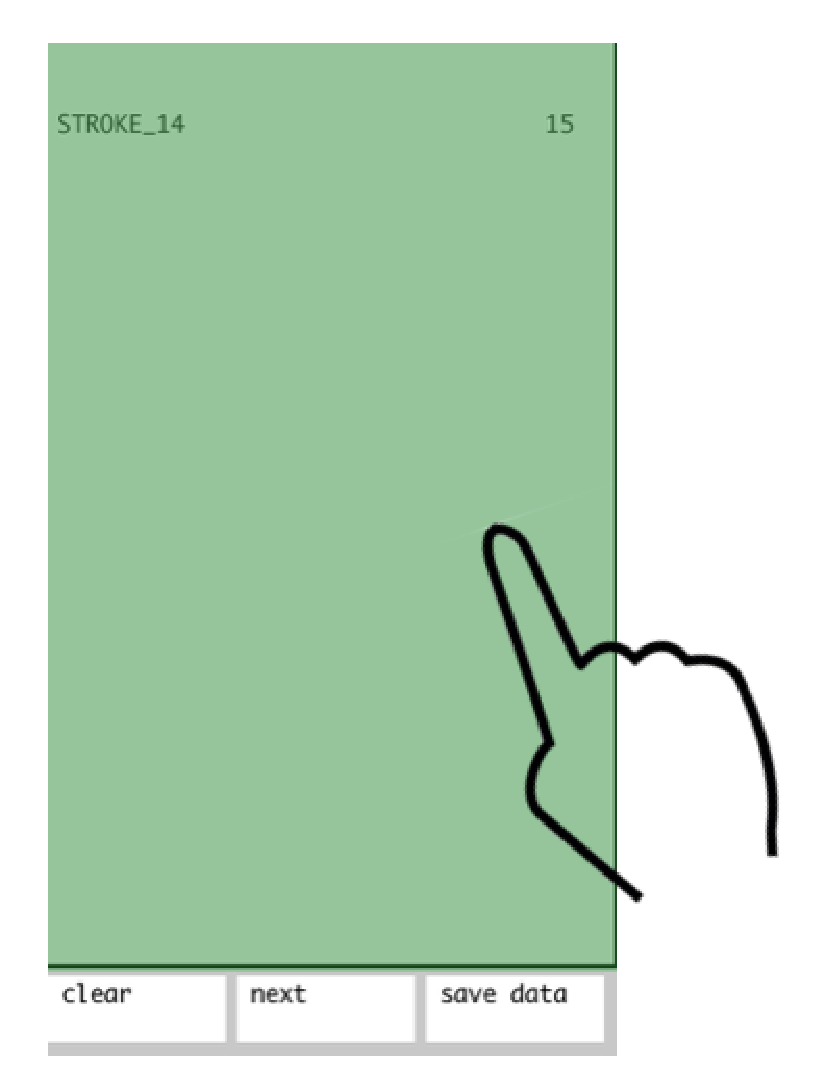
\includegraphics[width=0.4\columnwidth]{img/screenshot.eps}
\caption{The screen shot on the smartphone. The green area is the input area}
\label{fig:screenshot}
\end{figure}


\subsection{実験手順}
我々はまず,被験者に実験の目的を説明した.
その後,ユーザ調査において記入してもらった紙を見ながら,それぞれのジェスチャを入力するよう指示した.
ジェスチャは図\ref{fig:screenshot}における緑色の領域部分にジェスチャを入力するよう指示した.
その際,紙に書かれた,そのジェスチャを入力するときの姿勢に従い入力するよう指示した.
それぞれのジェスチャには,ジェスチャ番号がSTROKE\_1のようにして割り振られており,図\ref{fig:screenshot}に示すように,画面左上に入力すべきジェスチャが表示される.
タスクの1試行は被験者が1つのジェスチャを入力するまでである.被験者はランダムに選択されたそれぞれのジェスチャを1回ずつ入力し,これを1セッションとした.これを10セッション行った.被験者によって入力すべきジェスチャの数は異なるが,いずれの被験者においても20以上のジェスチャを入力する(20〜24個のジェスチャ,平均22個).したがって,被験者は平均して計220試行~(22ジェスチャ $\times$ 10セッション)行った.
ジェスチャが思うように入力できなかった場合には,何度でも書き直し可能とした.

\subsection{実験結果}
\TODO{あまり認識率が高くない結果を被験者ごとに載せる}

\TODO{認識速度はそこそこ速い結果を載せる}

\subsection{考察}
認識率が低かった原因を書く.
しかしながら,これまでのアルゴリズムにおいて,それぞれの特徴量は,認識に用いられるか用いられないかの二通りに分類され,閾値を設けることにより判別してきたが,同じ形状,同じ名前のジェスチャにおいても,学習に用いるデータによっては,認識に用いられる特徴量が異なる結果となる場合があった (閾値によって二通りのいずれかに分類されてしまうため,閾値の設定も難しいといった問題もある).また,図 1a において,「向き,位置」が認識に用いる特徴量として選ばれたが,「向き」は「位置」に比べ,学習データ間において,類似度が小さい組み合わせが存在するため,「向き」の方が「位置」よりも考慮されるべきではないのかという疑問や,それぞれの特徴量による類似度を,同じ尺度において扱うことができるのかという疑問があった (例えば,「大きさ」の類似度 0.9 と「向き」の類似度 0.9 は,同じくらい類似していると言えるのか).

\section{形状グループの作成}




%\begin{figure} [h!]
%	\begin{center}
%		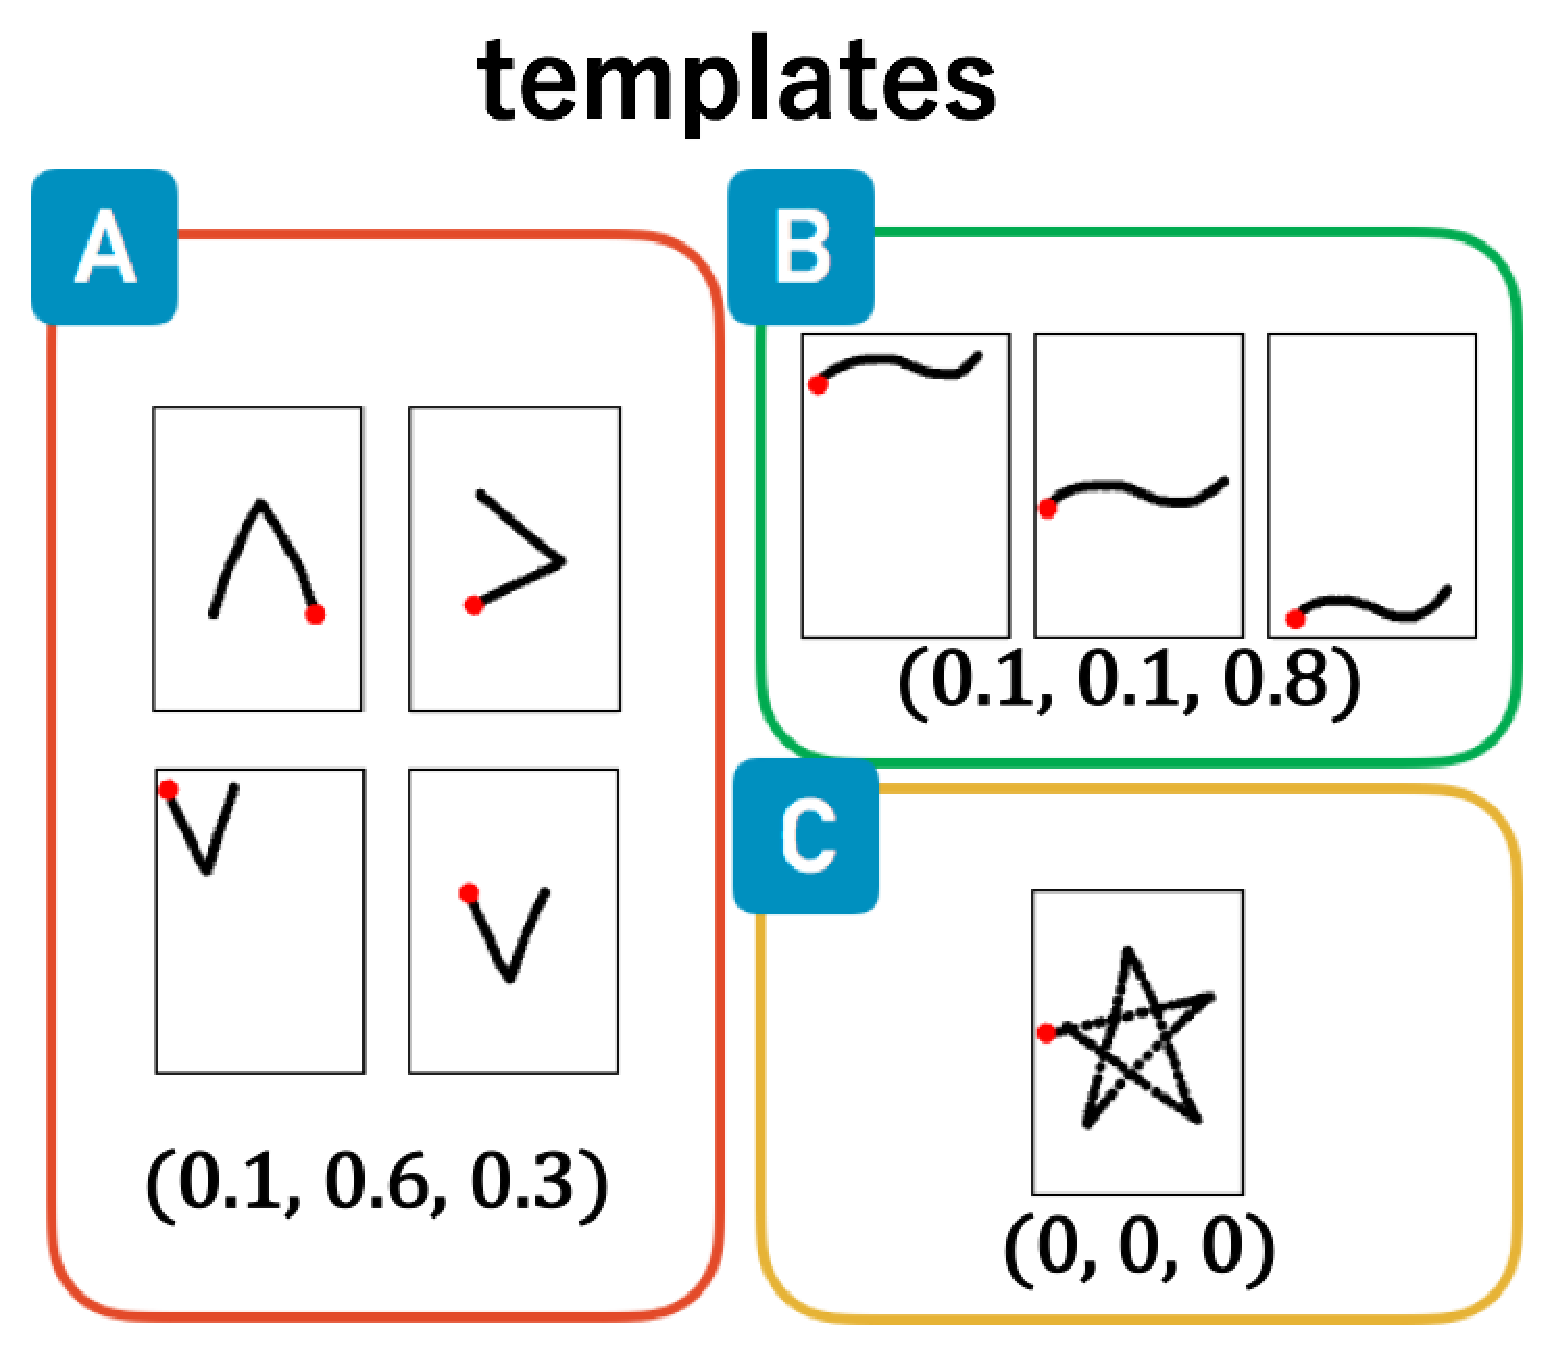
\includegraphics [width=0.7\hsize ]{img/group_weight.eps}
%	\end{center}
%	\caption{Examples of gesture groups and optimal weight values ($Ws$, $Wo$, $Wp$) for each group.}
%	\label{fig:group_weight}
%\end{figure}

\section{最適な重み付けのための実験}
\begin{figure} [h!]
	\begin{center}
		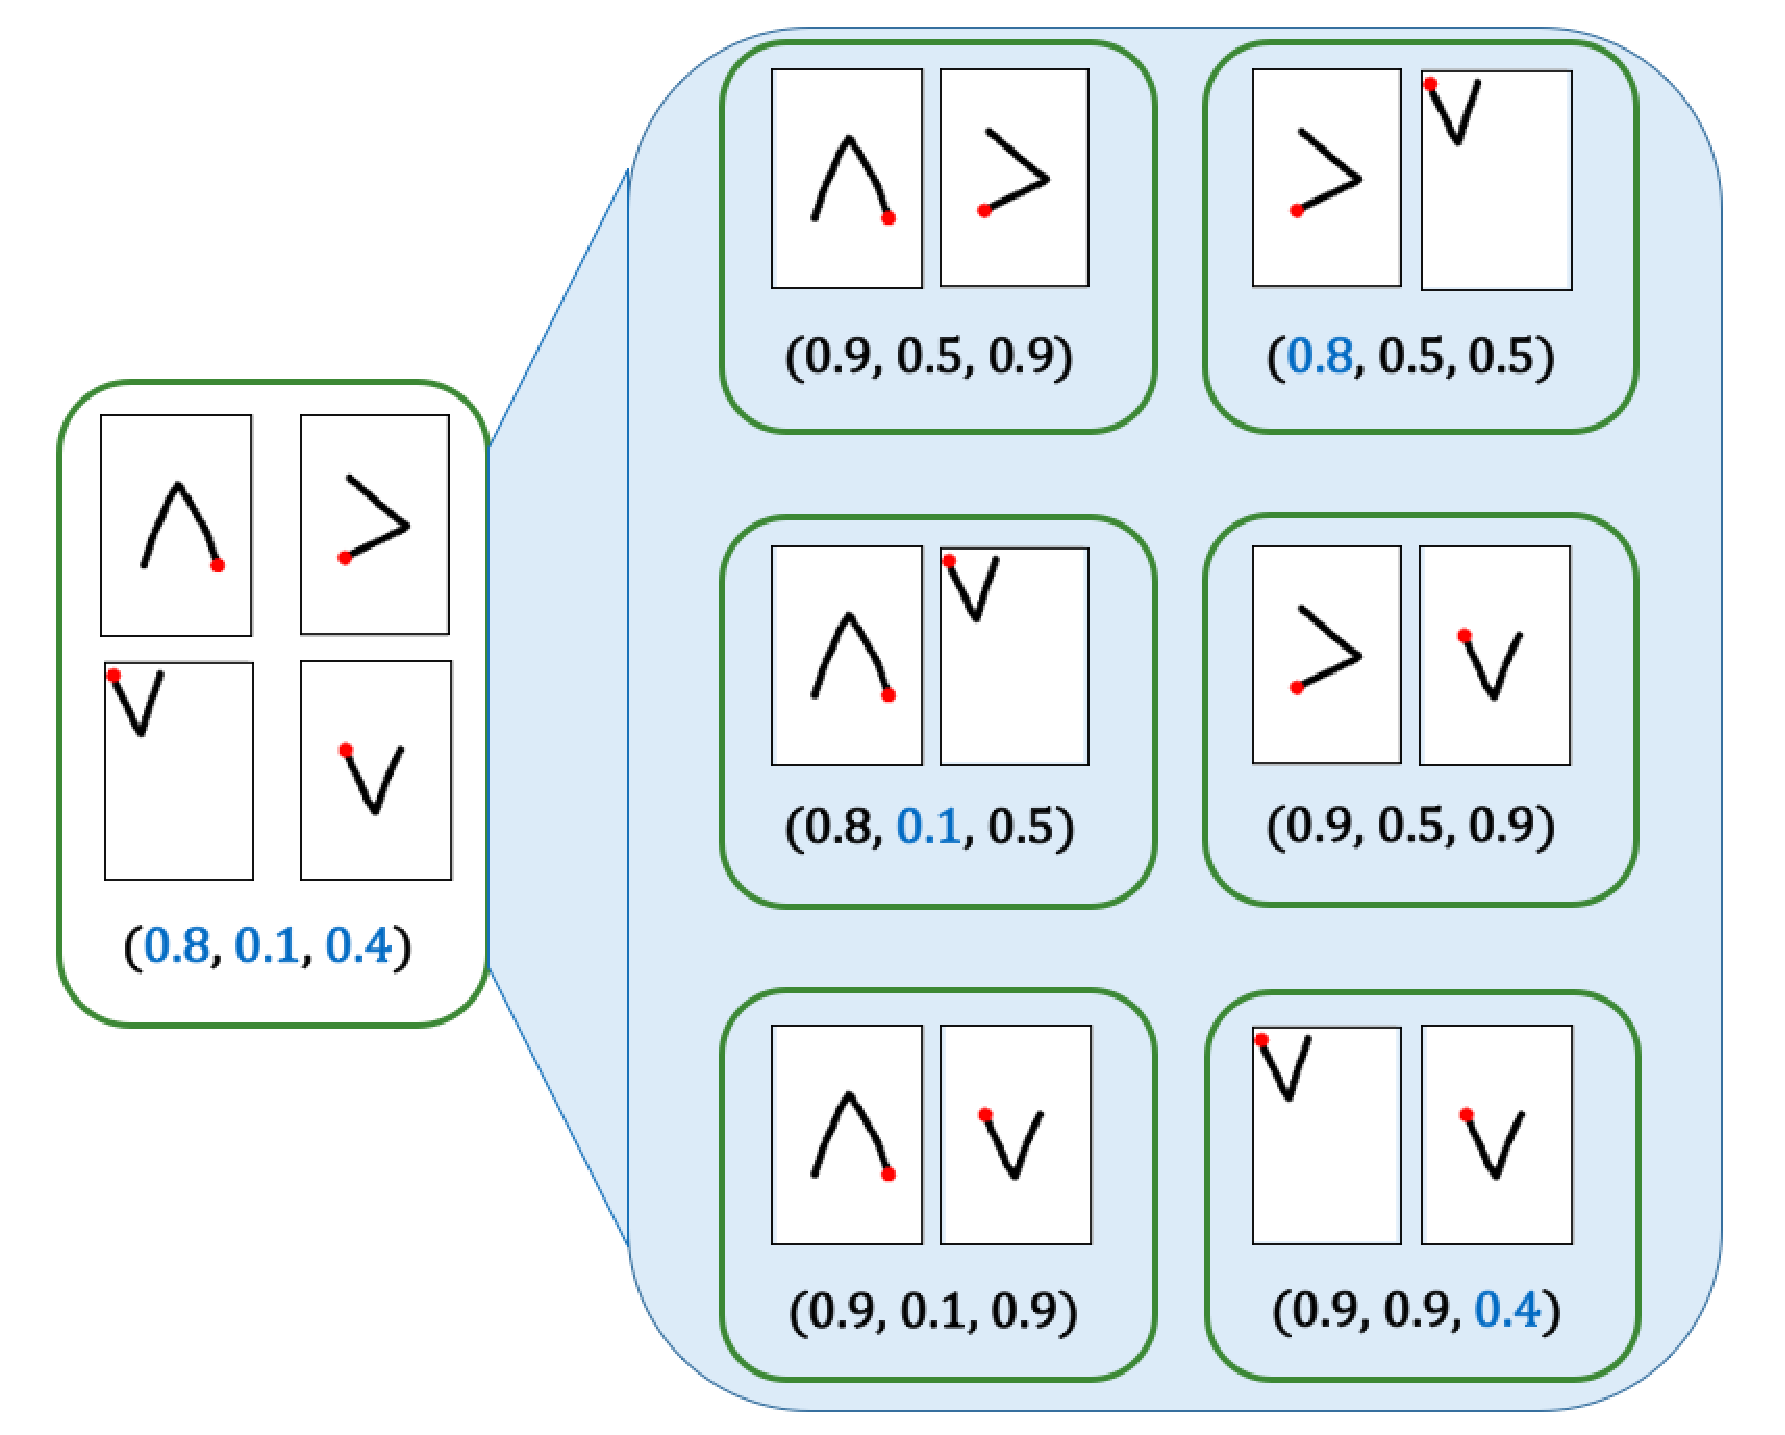
\includegraphics [width=0.8\hsize ]{img/group_similarity.eps}
	\end{center}
	\caption{An Example of how to decide a similarity ($Sts$, $Sto$, $Stp$) of tempaltes in a group gesture, in this case (0.8, 0.1, 0.4) is the similarities.}
	\label{fig:group_similarity}
\end{figure}

\begin{equation}
S{\tiny f} = S{\scriptsize cs} \times W{\scriptsize s} + S{\scriptsize co} \times W{\scriptsize o} + S{\scriptsize cp} \times W{\scriptsize p}
\end{equation}

\begin{figure} [h!]
	\begin{center}
		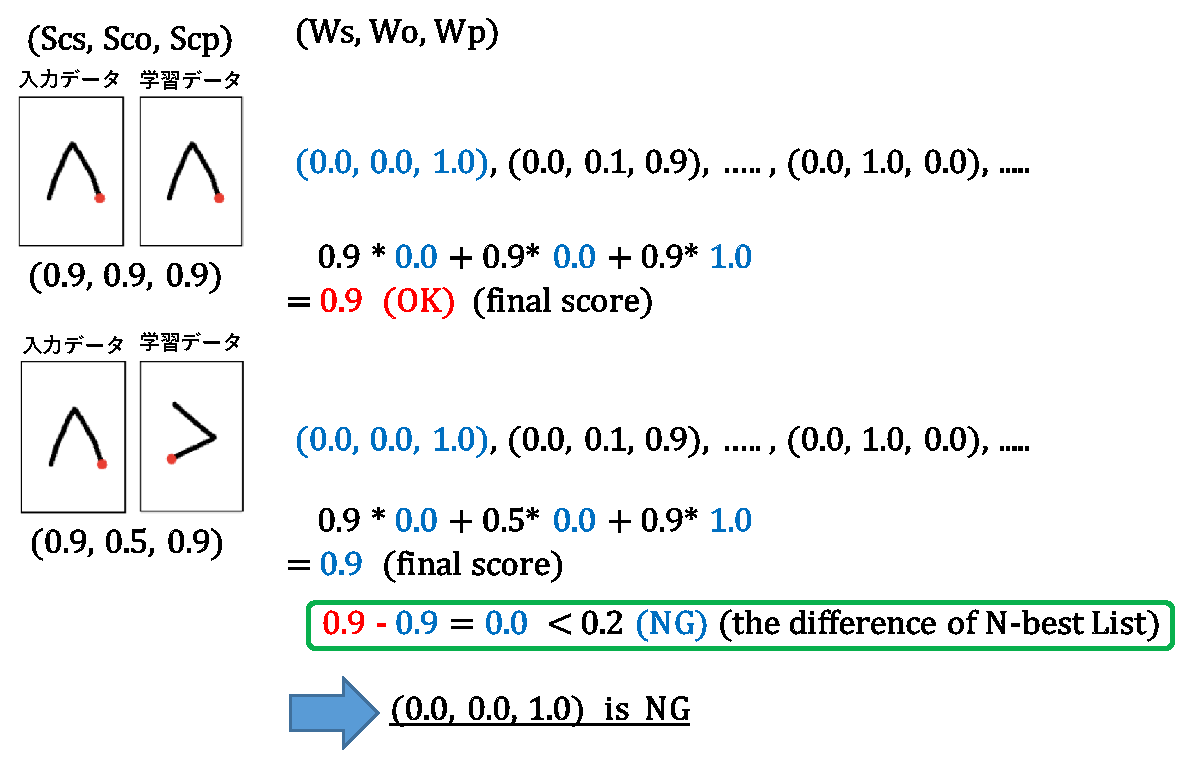
\includegraphics [width=0.8\hsize ]{img/weight_method1.eps}
	\end{center}
	\caption{The procedure to decide the optimal weight values }
	\label{fig:weight_method1}
\end{figure}

\begin{figure} [h!]
	\begin{center}
		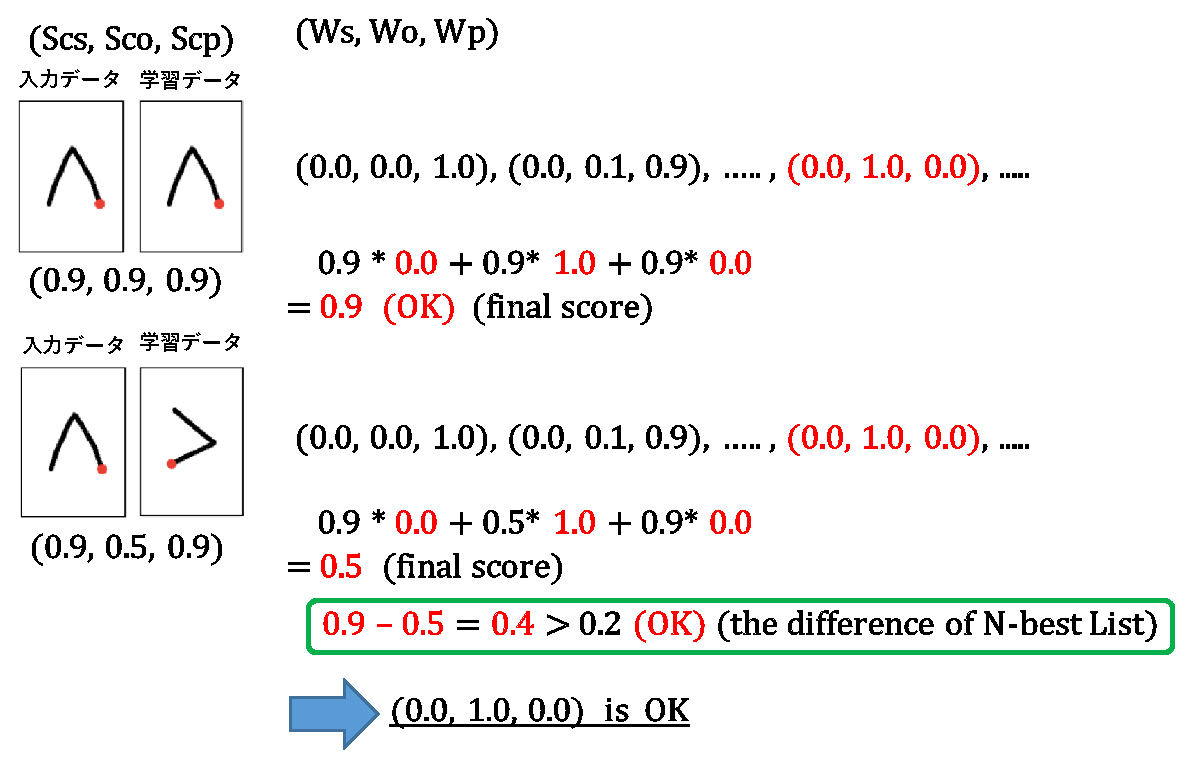
\includegraphics [width=0.8\hsize ]{img/weight_method2.eps}
	\end{center}
	\caption{The procedure to decide non optimal weight values}
	\label{fig:weight_method2}
\end{figure}

\subsection{実験結果}
\begin{figure*} [t]
 \begin{center}
  \includegraphics [width=1.0\columnwidth]{img/weight_graph.eps}
  \caption{The result of the experiment to find the optimal weight values, and blue lines indicates power approximation curves.}
  \label{fig:weight_graph}
 \end{center}
\end{figure*}

\section{ジェスチャの認識}


